\documentclass[12pt,titlepage]{article}
\usepackage[margin=1in]{geometry}
\usepackage{graphicx,amsmath,blindtext}

%% Variables definition
\newcommand{\vSubject}{Critical Thinking and Problem Solving}
\newcommand{\vSubtitle}{Combination Problems Mathematical, Probability and Decision Trees}
\newcommand{\vName}{Dicha Zelianivan Arkana}
\newcommand{\vNIM}{2241720002}
\newcommand{\vClass}{1i}
\newcommand{\vDepartment}{Information Technology}
\newcommand{\vStudyProgram}{D4 Informatics Engineering}

%% [START] Tikz related stuff
\usepackage{tikz}
\usetikzlibrary{svg.path,calc,shapes.geometric,shapes.misc}
\tikzstyle{terminator} = [rectangle, draw, text centered, rounded corners = 1em, minimum height=2.5em]
\tikzstyle{preparation} = [chamfered rectangle, chamfered rectangle sep=0.75em, draw, text centered, minimum height = 2em]
\tikzstyle{process} = [rectangle, draw, text centered, minimum height=2em]
\tikzstyle{decision} = [diamond, aspect=2, draw, text centered, minimum height=2em]
\tikzstyle{data}=[trapezium, draw, text centered, trapezium left angle=60, trapezium right angle=120, minimum height=2em]
\tikzstyle{connector} = [line width=0.25mm,->]
%% [END] Tikz related stuff

%% [START] Fancy header related stuff
\usepackage{fancyhdr}
\pagestyle{fancy}
\setlength{\headheight}{15pt} % compensate fancyhdr style
\fancyhead{}
\fancyfoot{}
\fancyfoot[L]{\thepage}
\fancyfoot[R]{\textit{\vSubject - \vSubtitle}}
\renewcommand{\footrulewidth}{0.4pt}% default is 0pt, overline for footer
%% [END] Fancy header related stuff

%% [START] Custom tabular command related stuff
\usepackage{tabularx}
\newcommand{\details}[2]{
    #1 & #2  \\
}
%% [END] Custom tabular command related stuff

%% [START] Figure related stuff
\newcommand{\image}[3][1]{
    \begin{figure}[h]
        \centering
        \includegraphics[#1]{#2}
        \caption{#3}
        \label{#3}
    \end{figure}
}
%% [END] Figure related stuff

\begin{document}
\begin{titlepage}
    \centering
    \vfill
    {\bfseries\LARGE
        \vSubject\\
        \vskip0.25cm
        \vSubtitle
    }
    \vfill
    \includegraphics[width=6cm]{images/polinema-logo.png}
    \vfill
    {
        \textbf{Name}\\
        \vName\\
        \vskip0.5cm
        \textbf{NIM}\\
        \vNIM\\
        \vskip0.5cm
        \textbf{Class}\\
        \vClass\\
        \vskip0.5cm
        \textbf{Department}\\
        \vDepartment\\
        \vskip0.5cm
        \textbf{Study Program}\\
        \vStudyProgram
    }
\end{titlepage}

\section*{Exercise}
\subsubsection*{Combination Problems Mathematical, Probability and Decision Trees}
There are two ways I go to work, both involve a two part journey.
\begin{itemize}
    \item I can cycle to the bus stop; it usually takes 5 minutes, or 15 minutes if the railroad crossing is closed on the road, which happens on 10\% of occasions.
    \item A bus takes an average of 5 minutes to arrive. I took the first bus, which may have been a slow bus that took 30 minutes or a fast bus that took 15 minutes. Chances of I get a slow bus is 20\%
    \item Or, I could drive to the Park and Ride parking lot
    \item Driving normally takes 15 minutes, but about half the time there is a traffic jam and it taks 20 minutes.
    \item When I get to the Park and Ride, sometimes I get the bus right away, but there's a 60\% chance I'll have to wait 10 minutes for the next bus.
    \item The bus took 10 minutes to take me to work.
\end{itemize}

\subsubsection*{Questions}
\begin{enumerate}
    \item {
        What is my shortest time to start to work?

        From the statements above, we can gather up these informations:
        \begin{enumerate}
            \item {
                The First Route
                \begin{itemize}
                    \item Cycle: 5 minutes
                    \item Bus: 0 minutes
                    \item Fast Bus: 15 minutes
                \end{itemize}
                \textbf{Total}: 20 minutes
                }
                \item {
                    The Second Route
                    \begin{itemize}
                        \item Drive: 15 minutes
                        \item Wait for a Bus: 0 minutes
                        \item Riding the Bus: 10 minutes
                    \end{itemize}
                \textbf{Total}: 25 minutes
            }
        \end{enumerate}
        Based on the data that we've summarised, the shorted path would be the first one because it only takes 20 minutes to travel.
    }
    \pagebreak
    \item {
        On average, what is my best option for going to work and how much time do I need?

        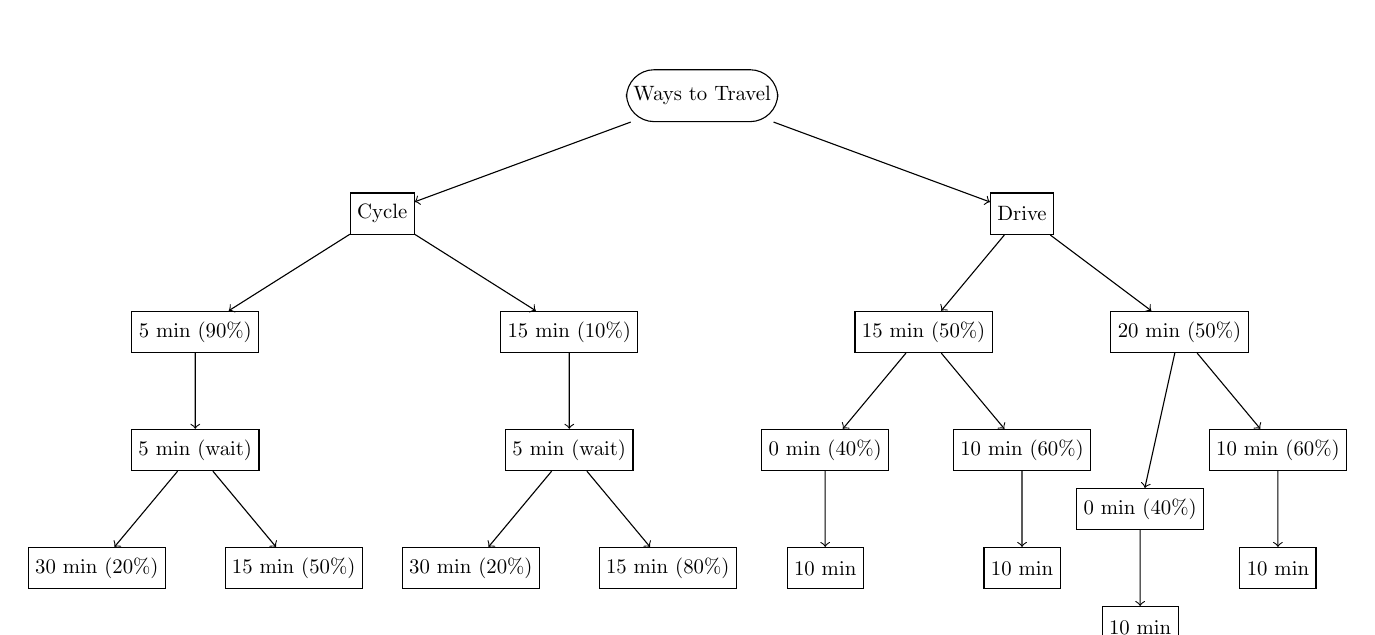
\begin{tikzpicture}[every path/.style={->},every child/.style={sibling distance=2.5cm},every node/.style={scale=0.75}]
            \node[terminator] {Ways to Travel}
                child {node[process,xshift=-3.75cm] {Cycle}
                    child {node[process,xshift=-1.5cm] {5 min (90\%)}
                        child {node[process] {5 min (wait)}
                            child {node[process] {30 min (20\%)}}
                            child {node[process] {15 min (50\%)}}}}
                    child {node[process,xshift=1.5cm] {15 min (10\%)}
                        child {node[process] {5 min (wait)}
                            child {node[process] {30 min (20\%)}}
                            child {node[process] {15 min (80\%)}}}}}
                child {node[process,xshift=3.75cm] {Drive}
                    child {node[process] {15 min (50\%)}
                        child {node[process] {0 min (40\%)}
                            child {node[process] {10 min}}}
                        child {node[process] {10 min (60\%)}
                            child {node[process] {10 min}}}}
                    child {node[process,xshift=1cm] {20 min (50\%)}
                        child {node[process,yshift=-1cm,xshift=1cm] {0 min (40\%)}
                            child {node[process] {10 min}}}
                        child {node[process] {10 min (60\%)}
                            child {node[process] {10 min}}}}};
        \end{tikzpicture}

        To find the most efficient option, we need to try each path and then multiply the number of minutes with the number of the percentages.
        We can then list them as such:
        \begin{itemize}
            \item {
                \textbf{Cycle}
                \begin{enumerate}
                    \item {
                        First Path
                        \begin{itemize}
                            \item $90\% \times 5 = 4.5~minutes$
                            \item $5~minutes$
                            \item $20\% \times 30 = 6~minutes$
                            \item \textbf{Total:} 15.5~minutes
                        \end{itemize}
                    }
                    \item {
                        Second Path
                        \begin{itemize}
                            \item $90\% \times 5 = 4.5~minutes$
                            \item $5~minutes$
                            \item $50\% \times 15 = 7.5~minutes$
                            \item \textbf{Total:} 17~minutes
                        \end{itemize}
                    }
                \end{enumerate}
            }
            \item {
                \textbf{Drive}
                \begin{enumerate}
                    \item {
                        First Path
                        \begin{itemize}
                            \item $50\% \times 15 = 7.5~minutes$
                            \item $40\% \times 0 = 0$
                            \item 10 minutes
                            \item \textbf{Total:} 17.5 minutes
                        \end{itemize}
                    }
                    \item {
                        Second Path
                        \begin{itemize}
                            \item $50\% \times 15 = 7.5~minutes$
                            \item $60\% \times 10 = 6~minutes$
                            \item 10 minutes
                            \item \textbf{Total:} 23.5 minutes
                        \end{itemize}
                    }
                    \pagebreak
                    \item {
                        Third Path
                        \begin{itemize}
                            \item $50\% \times 20 = 10~minutes$
                            \item $40\% \times 0 = 0~minutes$
                            \item 10 minutes
                            \item \textbf{Total:} 20 minutes
                        \end{itemize}
                        }
                        \item {
                            Fourth Path
                        \begin{itemize}
                            \item $50\% \times 20 = 10~minutes$
                            \item $60\% \times 10 = 6~minutes$
                            \item 10 minutes
                            \item \textbf{Total:} 26 minutes
                        \end{itemize}
                    }
                \end{enumerate}
            }
        \end{itemize}
        From the list above, we can conclude that using the bicycle is the fastest and it took 15.5 minutes.
    }
    \item {
        What is the probability that the first trip option takes 40 minutes or more?

        To calculate this, we can look at the branches where the total time is 40 minutes or more and add the probabilities.
        There are:
        \begin{itemize}
            \item 18\% (for 40 minutes)
            \item 2\% (for 50 minutes)
            \item \textbf{Total:} 20\%.
        \end{itemize} 
        In conclusion, the probability of the first trip option taking 40 minutes or more is 20\%
    }
\end{enumerate}

\end{document}

